%!TEX root=paper.tex
\newcommand{\picscale}{0.45}
\newcommand{\yunit}{0.5}
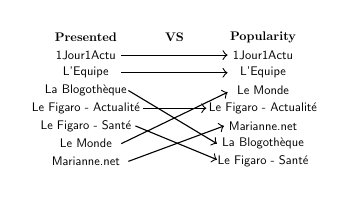
\begin{tikzpicture}[scale=\picscale, every node/.style={scale=\picscale},font=\sffamily]
    % Columns.
    \node at (0  , 0) {\bf Presented};
    \node at (2.5, 0) {\bf VS};
    \node at (5  , 0) {\bf Popularity};
    
    % As presented.
    \node at (0,-1*\yunit) {1Jour1Actu};
    \node at (0,-2*\yunit) {L'Equipe};
    \node at (0,-3*\yunit) {La Blogoth\`{e}que};
    \node at (0,-4*\yunit) {Le Figaro - Actualit\'{e}};
    \node at (0,-5*\yunit) {Le Figaro - Sant\'{e}};
    \node at (0,-6*\yunit) {Le Monde};
    \node at (0,-7*\yunit) {Marianne.net};
    
    % As popular.
    \node at (5,-1*\yunit) {1Jour1Actu};
    \node at (5,-2*\yunit) {L'Equipe};
    \node at (5,-3*\yunit) {Le Monde};
    \node at (5,-4*\yunit) {Le Figaro - Actualit\'{e}};
    \node at (5,-5*\yunit) {Marianne.net};
    \node at (5,-6*\yunit) {La Blogoth\`{e}que};
    \node at (5,-7*\yunit) {Le Figaro - Sant\'{e}};
    
    % Arrows between presented and popular.
    \draw [->] (1,-1*\yunit)   --   (4,-1*\yunit);
    \draw [->] (1,-2*\yunit)   --   (4,-2*\yunit);
    \draw [->] (1.2,-3*\yunit) --   (3.7,-6*\yunit);
    \draw [->] (1.6,-4*\yunit) --   (3.4,-4*\yunit);
    \draw [->] (1.4,-5*\yunit) --   (3.7,-6.9*\yunit);
    \draw [->] (1,-6*\yunit)   --   (4,-3.1*\yunit);
    \draw [->] (1.2,-7*\yunit) --   (3.9,-5*\yunit);
    
\end{tikzpicture} 